\subsection{GUI}

GUIs are not used in HPC as they use memory and slow down computations and are generally not necessary as all the interactions with HPC machines is done through a command line.
However, our group has chosen to code in Java, and GUI is one of Java's strengths as it should look the same on every machine. So it was decided that we are not taking advantages of our chosen language unless we create a GUI. 
GUI created is responsible for the input parameters of the simulation. Initially, it would just take the values and run the simulation.
%\begin{figure} [BeforeRange]
%\begin{center}
%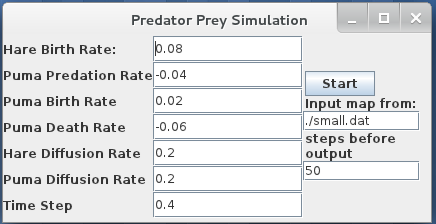
\includegraphics[scale = 0.5]{figs/BeforeRange.png}
%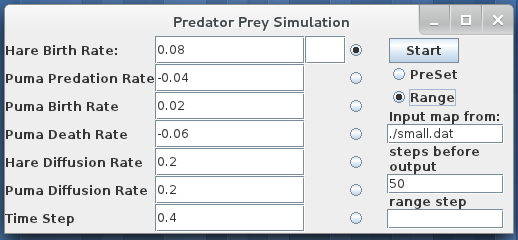
\includegraphics[scale = 0.47]{figs/WithRange.png}
%\caption{GUI: Initial version and final version}
%\label{fig:BeforeRange}
%\end{center}
%\end{figure}
However, in later) versions, \emph{range} option was added to be able to run multiple simulations changing one of the parameters.
% (see fig. \ref{fig:BeforeRange}).
The frame is divided into three parts (all on separate frames): input, input2, button.
% (see fig. \ref{fig:input}).
Input holds labels and text fields for parameter inputs. 
%\begin{figure} [input]
%\begin{center}
%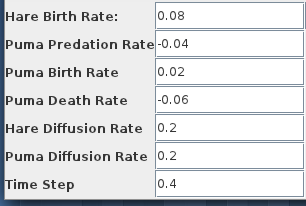
\includegraphics[scale = 0.5]{figs/input.png}
%
\includegraphics[scale = 0.5]{figs/input2.png}
%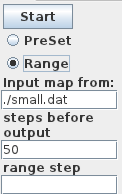
\includegraphics[scale = 0.5]{figs/button.png}
%\caption{Panels: input, input2, button}
%\label{fig:input}
%\end{center}
%\end{figure}
Input2 holds second text field and radio buttons to chose which parameter to range over, is not visible unless range is selected. 
Button holds start button, choice between range and preset values and parameter values that are general like input file, steps before output.
GUI is still very simplistic and could be enhanced more but was not due to time constraints.
